\chapter{Parameters and Optimization}
\label{ch:parameters}

\epigraph{Far better an approximate answer to the right question \ldots\ than an exact answer to the wrong question.}{--- John Tukey}

\lettrine[lines=2]{T}{he model} employs a three-tier parameter hierarchy comprising 109 parameters, partitioned into three Python dataclass objects that mirror their distinct roles.

% ======================================================================
\section{Parameter Categories}
\label{sec:param-categories}

\texttt{ModelParameters} encapsulates 4 infrastructure-level settings---tumor volume (from which the grid dimension is derived via Equation~\ref{eq:grid_dim}), block size (default $10\;\mu\text{m}$), random seed, and maximum step count---that are fixed by the modeler and do not vary across patient cases. \texttt{PatientParameters} encodes 18 clinical variables specific to each individual: biological sex, BMI, treatment regimen, treatment start time, and 13 immune cell concentrations read directly from the ARON-1 dataset. \texttt{WeightParameters} contains the 87 biological rate constants and probability thresholds governing all agent behaviors, from tumor proliferation to drug effectiveness. These weight parameters are the target of Bayesian optimization, as they represent quantities that cannot be measured directly from patient data and must be inferred by calibrating the model against observed clinical outcomes.

% ======================================================================
\section{Weight Parameters}
\label{sec:weight-params}

The 87 weight parameters control probability thresholds and scaling factors for all agent behaviors, organized by cell type. These parameters are optimized via Bayesian methods to match clinical trial outcomes. Table~\ref{tab:param-summary} provides a high-level overview; the complete per-parameter listings with defaults and descriptions are given in Appendix~\ref{ch:appendix-params}.

\begin{table}[htbp]
\centering
\caption{Summary of weight parameters by category.}
\label{tab:param-summary}
\begin{adjustbox}{max width=\textwidth}
\begin{tabular}{@{}lclp{5.8cm}@{}}
\toprule
\textbf{Category} & \textbf{Count} & \textbf{Description} & \textbf{Example Parameters} \\
\midrule
M1 Macrophage & 9 & Pro-inflammatory macrophage behavior & \texttt{w\_m1\_phagocytosis}, \texttt{w\_m1\_t\_kill\_rate} \\
M2 Macrophage & 6 & Anti-inflammatory macrophage behavior & \texttt{w\_m2\_tumor\_growth}, \texttt{w\_m2\_angiogenesis} \\
Tumor Cell & 12 & Tumor growth, apoptosis, and immune evasion & \texttt{w\_tumor\_growth\_eff}, \texttt{w\_gene\_pd1\_inhibition} \\
CD4+ T Cell & 13 & Helper T cell differentiation and spawning & \texttt{w\_cd4\_treg\_diff\_effect}, \texttt{w\_cd4\_th1\_spawn\_m1} \\
Cytotoxic T Cell & 7 & CD8+ killing, proliferation, and PD-1 response & \texttt{w\_cytotoxic\_kill}, \texttt{w\_cytotoxic\_pd1\_inhibition} \\
Mast Cell & 6 & Angiogenesis, immune modulation, DC spawning & \texttt{w\_mast\_cell\_angiogenesis}, \texttt{w\_mast\_cell\_spawn\_dc} \\
NK Cell & 3 & Natural killer direct and indirect cytotoxicity & \texttt{w\_natural\_killer\_kill\_rate}, \texttt{w\_nkl\_t\_kill\_rate} \\
pDC & 7 & Dendritic cell immune orchestration & \texttt{w\_pdc\_nkl\_spawn}, \texttt{w\_pdc\_t\_kill} \\
Treg & 5 & Regulatory T cell immunosuppression & \texttt{w\_treg\_t\_kill\_rate}, \texttt{w\_treg\_activation} \\
Global & 11 & Simulation-wide thresholds and drug effects & \texttt{w\_ici\_effectiveness}, \texttt{w\_cell\_base\_death\_prob} \\
Glucose & 8 & Metabolic microenvironment dynamics & \texttt{w\_glucose\_diffusion}, \texttt{w\_glucose\_tumor\_consumption} \\
\midrule
\textbf{Total} & \textbf{87} & \multicolumn{2}{l}{\textit{79 cell-type + 8 glucose = 87 optimizable weights}} \\
\bottomrule
\end{tabular}
\end{adjustbox}
\end{table}

% ======================================================================
\section{Glucose Parameters}
\label{sec:glucose-params}

The glucose microenvironment system introduces 8 weight parameters, all prefixed with \texttt{w\_glucose\_}. These parameters control the physical dynamics of glucose diffusion, the metabolic consumption rates, and the coupling between glucose availability and agent behavior (see Appendix~\ref{ch:appendix-params} for the full table).

\paragraph{Parameter Interactions.}

The glucose parameters interact with existing weights through three coupling mechanisms. Tumor cell duplication probability is multiplied by a glucose factor $\min(1, C \cdot \param{w\_glucose\_\allowbreak growth\_sensitivity})$, suppressing growth when glucose is depleted. Immune cell kill rates and activation probabilities are analogously scaled by \param{w\_glucose\_immune\_\hspace{0pt}sensitivity}, coupling metabolic availability to immune effectiveness. The balance between \param{w\_glucose\_\allowbreak source\_rate} (vascular supply) and \param{w\_glucose\_\allowbreak tumor\_consumption} (tumor demand) determines the spatial glucose profile, with high consumption creating depletion zones that impair both tumor growth and immune infiltration.

% ======================================================================
\section{Bayesian Optimization}
\label{sec:bayesian-optimization}

Optimizing 87 weight parameters precludes naive strategies: grid search with 3 values per parameter would require $3^{87}$ evaluations, and random search is inefficient in high-dimensional correlated spaces. Bayesian optimization addresses this by constructing a probabilistic surrogate model that guides sampling toward promising regions. The Tree-structured Parzen Estimator (TPE) algorithm progressively concentrates evaluations where improvement is most likely, which is essential given that each trial requires a full simulation for every patient in the clinical dataset.

\subsection{Framework}

The model uses Optuna~\cite{optuna} for Bayesian hyperparameter optimization. Optuna's TPE sampler implements the surrogate-based strategy described above, efficiently exploring the 87-dimensional weight space by building and refining probabilistic models of the objective function landscape at each trial.

\subsection{Objective Function}

The optimization objective is to minimize the prediction error of the model against the ARON-1 clinical dataset. For each Optuna trial, the following process is executed:

\begin{enumerate}
    \item A set of weight parameters is suggested by the TPE sampler within predefined bounds.
    \item For each patient case in the ARON-1 dataset, a simulation is run with the patient's clinical features (sex, BMI, treatment, immune cell concentrations) and the suggested weight parameters.
    \item The simulation outcome (survival/death, number of steps) is compared against the clinical outcome.
    \item The per-case error is computed as:
    \begin{equation*}
        \text{error}_i = \begin{cases}
            (\text{steps}_i - \text{OS}_i)^2 & \text{if prediction matches outcome} \\
            \text{HIGH\_PENALTY}^2 & \text{if prediction contradicts outcome}
        \end{cases}
    \end{equation*}
    where $\text{OS}_i$ is the observed overall survival (in steps) and $\text{HIGH\_PENALTY} = 500$.
    \item The trial objective value is the mean error across all cases.
\end{enumerate}

\subsection{Search Space}

The search space, defined in the \texttt{suggest\_parameters()} function, covers all 87 weight parameters. The 62 positive weights are sampled log-uniformly in $[0.25, 4.0]$, ensuring symmetric exploration of multiplicative scaling factors, while the 15 bias parameters are sampled uniformly in $[-1.0, 1.0]$. Drug effectiveness weights (\param{w\_ici\_effectiveness}, \param{w\_tki\_effectiveness}) range over $[0.0, 1.0]$, and threshold weights use domain-specific bounds: \param{w\_tumor\_\allowbreak growth\_threshold} in $[0.75, 0.99]$, \param{w\_cell\_base\_\allowbreak death\_prob} in $[0.001, 0.1]$, and \param{w\_progressive\_\allowbreak exhaustion} in $[0.005, 0.3]$. The integer parameter \texttt{receptor\_threshold\_variation} takes values in $\{0, 1, 2, 3\}$. The 8 glucose parameters have individually constrained ranges respecting physical constraints---notably, \texttt{w\_glucose\_diffusion} is bounded by $[0.01, 0.16]$ to satisfy the $D < 1/6$ numerical stability requirement---while consumption, sensitivity, and chemotaxis parameters span ranges calibrated to produce biologically plausible glucose field dynamics.

\begin{keyinsight}
Log-uniform sampling for positive weights ensures that the optimizer explores multiplicative scaling factors symmetrically: halving and doubling a weight receive equal prior probability.  This is appropriate because many biological rate parameters span orders of magnitude, and uniform sampling would over-represent values near the upper bound.
\end{keyinsight}

\subsection{Optimization Configuration}

The optimization runs for $N = 250$ trials, each evaluating every patient case in the ARON-1 dataset. Training uses \texttt{MPI.COMM\_SELF} to create isolated single-rank model instances, avoiding MPI communication overhead during optimization. Trial errors and the best-so-far error are logged to \texttt{data/trial\_errors.csv} for convergence analysis.


% ======================================================================
\section{Clinical Dataset}
\label{sec:clinical-dataset}

\subsection{ARON-1 Study}

The ARON-1 study is a clinical trial of advanced renal cell carcinoma patients treated with immune checkpoint inhibitors (ICI), tyrosine kinase inhibitors (TKI), or their combination~\cite{santoni2024}. The dataset provides the ground truth against which the model is calibrated.

\subsection{Dataset Structure}

The clinical dataset is stored in \texttt{src/learning/data/ARON.csv} and contains, for each patient case, demographic features (sex, BMI), treatment type (ICI, TKI, or ICI+TKI), 13 immune cell concentration measurements matching the \param{Patient\-Parameters} fields, and outcome data (overall survival in time units and a binary death indicator). Each row parameterizes a simulation run during optimization, with the patient's clinical features passed as keyword arguments to \texttt{RCCModel} and the simulation's survival prediction compared against the clinical outcome to compute the trial error.

% ============================================================================
\section{Parameter Sensitivity Analysis}
\label{sec:parameter_sensitivity}
% ============================================================================

Figure~\ref{fig:parameter_sensitivity} demonstrates the sensitivity of simulation outcomes to key parameter variations within the defined ranges. This analysis identifies which parameters have the strongest influence on tumor dynamics and treatment efficacy, providing guidance for parameter selection and model robustness assessment.

\begin{figure}[htbp]
\centering
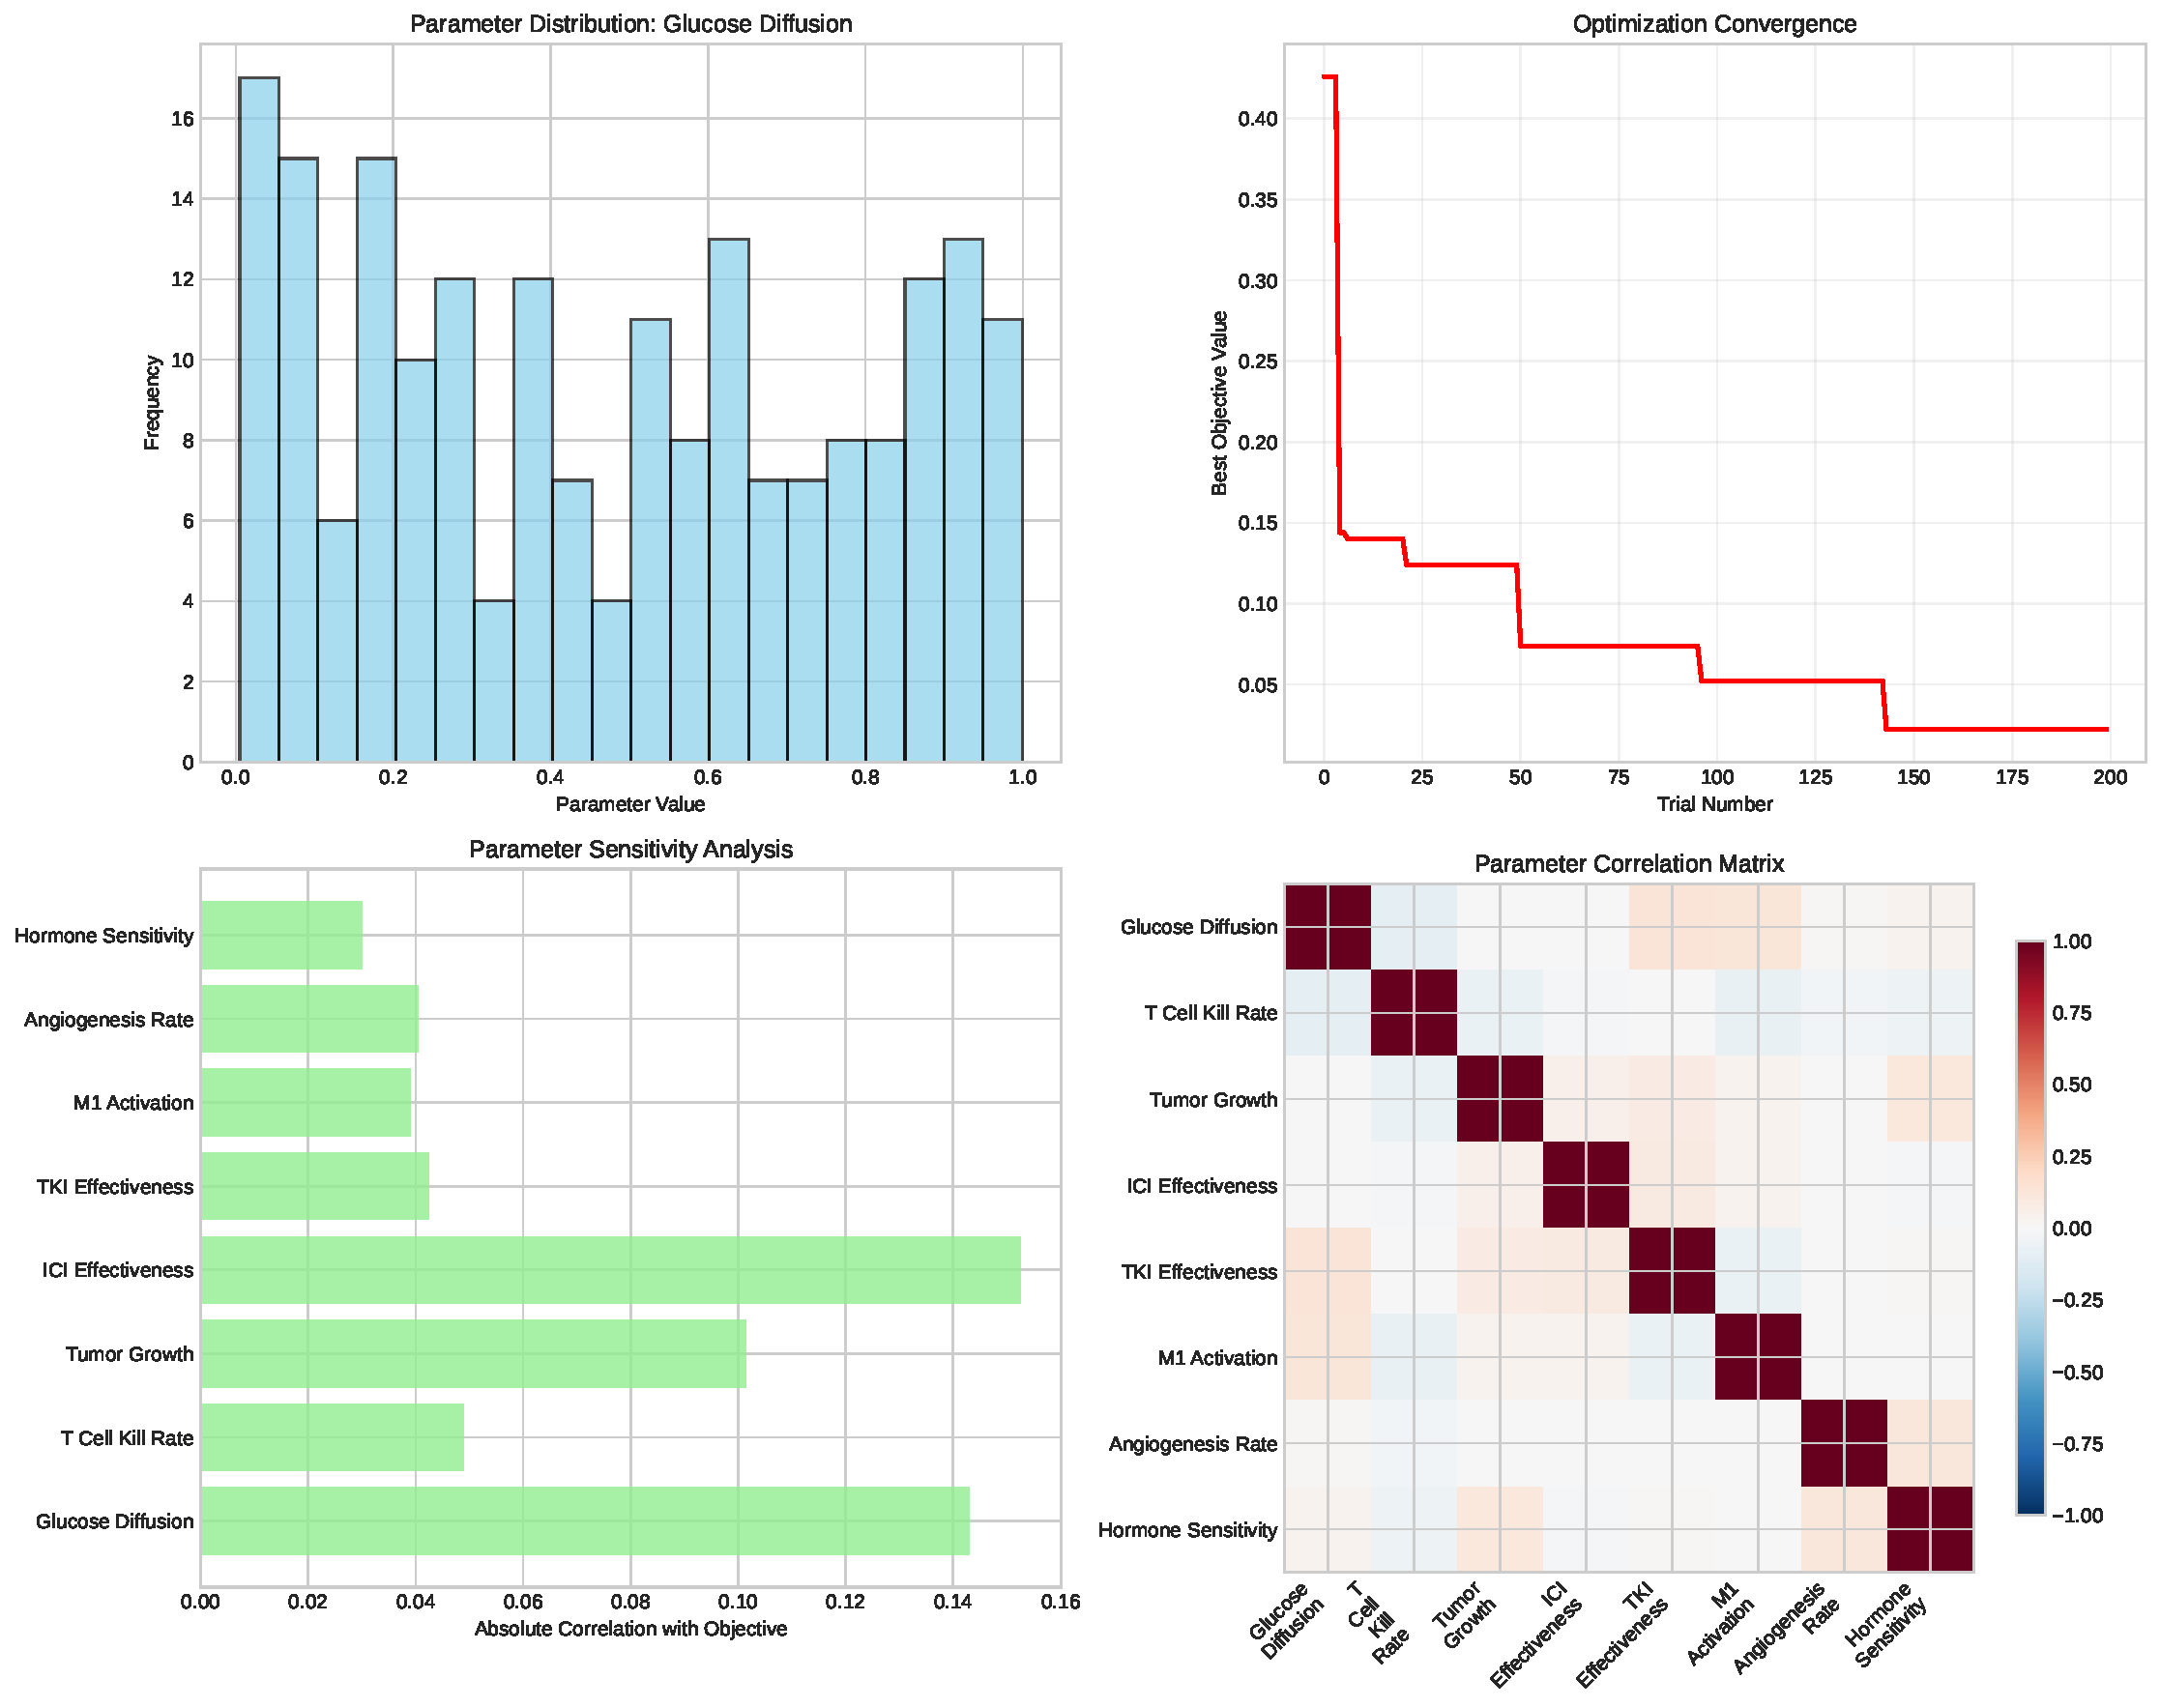
\includegraphics[width=0.85\textwidth]{figures/parameter_sensitivity.pdf}
\caption{Parameter sensitivity analysis showing the impact of key model parameters on tumor cell population dynamics. The analysis varies parameters within their defined ranges while keeping others at baseline values. Most sensitive parameters include glucose consumption rates, treatment effectiveness weights, and immune cell interaction parameters. Error bars represent variance across multiple simulation runs.}
\label{fig:parameter_sensitivity}
\end{figure}

The next chapter presents simulation results and validates the calibrated model against ARON-1 clinical data.
